\documentclass[10pt]{beamer}

\usetheme{m}

\usepackage{booktabs}
\usepackage[scale=2]{ccicons}

\usepackage{multicol}

\usepackage{pgfplots}
\usepgfplotslibrary{dateplot}

\usepackage{upgreek}


 
\newtheorem{examplenegative}{exampleblock}
\newenvironment<>{examplenegative}[1]{%
  \setbeamercolor{block title example}{fg=red}%
  \begin{exampleblock}#2{#1}}{\end{exampleblock}}


\setbeamercovered{invisible}

%Notes on laptop but not on presentation
%\usepackage{pgfpages}
%\setbeameroption{show notes}
%\setbeameroption{show notes on second screen=right}
%\setbeameroption{show notes on second screen}

\usepackage[]{algorithm2e}

\title{App-udvikling}
\subtitle{2. Lektion}
\date{\today}
\author{Sune Sylvest Nilausen}
%\institute{Institute or miscellaneous information}
% \titlegraphic{\hfill\includegraphics[height=1.5cm]{logo/logo}}
\graphicspath{ {../} }

\begin{document}
%\setbeamertemplate{caption}{\raggedright\insertcaption\par}

\maketitle

\begin{frame}
  \frametitle{Indholdsfortegnelse}
  \setbeamertemplate{section in toc}[sections numbered]
  \tableofcontents[hideallsubsections]
\end{frame}

\section{Opsummering fra sidst}

\begin{frame}{Iterativ og Agil}
\begin{figure}	
		\centering
		\includegraphics[width=\linewidth]{img/sprints.jpg}
		\caption{Agil arbejdsprocess i flere iterationer.}
	\end{figure}
\end{frame}

\section{Design}
\begin{frame}{Mennesker Aktiviteter Kontekst}
		\centering
	\includegraphics[width=.45\linewidth]{img/elderly.jpg}\quad%
	\includegraphics[width=.45\linewidth]{img/running.jpg}\quad%
	\includegraphics[width=.45\linewidth]{img/people.jpg}\quad%
	\includegraphics[width=.45\linewidth]{img/smartphones_inclass}
\end{frame}

\begin{frame}{Design Principper: Nærhed og Mønstre}
\centering
	\includegraphics[width=.45\linewidth]{img/norepetitionexample.png}\quad%
	\includegraphics[width=.45\linewidth]{img/repetitionexample.png}\quad%
	\includegraphics[width=.45\linewidth]{img/noproximityexample.png}\quad%
	\includegraphics[width=.45\linewidth]{img/proximityexample.png}
\end{frame}

\begin{frame}{Design Principper: Opstilling og Kontrast}
\centering
	\includegraphics[width=.45\linewidth]{img/noalignmentexample.png}\quad%
	\includegraphics[width=.45\linewidth]{img/alignmentexample.png}\quad%
	\includegraphics[width=.45\linewidth]{img/nocontrastexample.png}\quad%
	\includegraphics[width=.45\linewidth]{img/contrastexample.png}
\end{frame}

\begin{frame}{Design Principper: Størrelse og Adskillelse}
 \centering
	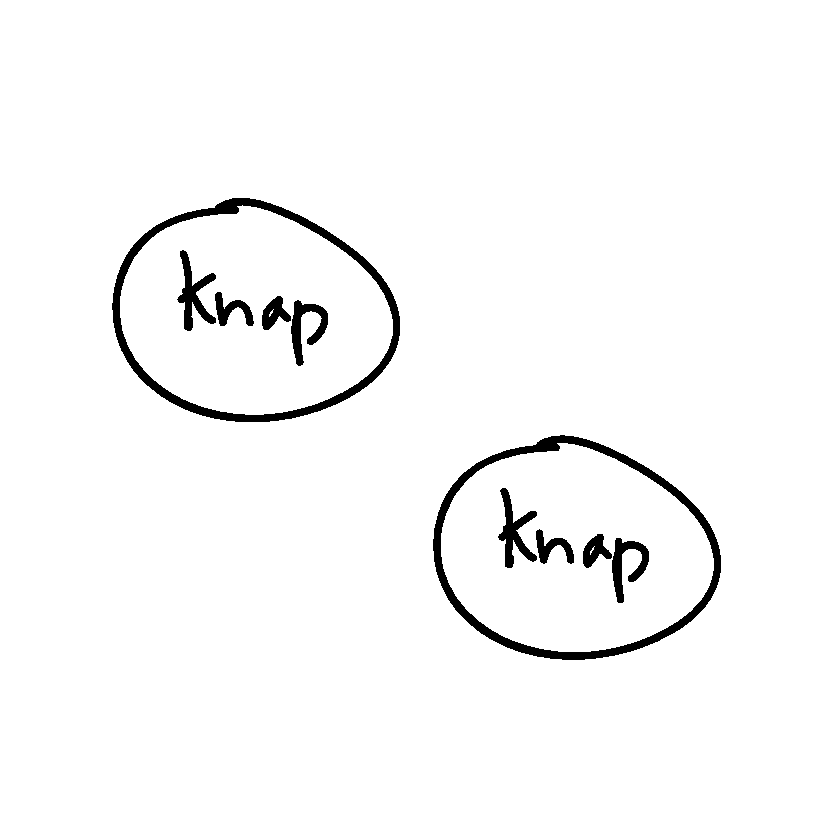
\includegraphics[scale=0.31]{img/sizeuden.pdf}\quad%
	
\includegraphics[scale=0.31]{img/sizemed.pdf}\quad%
	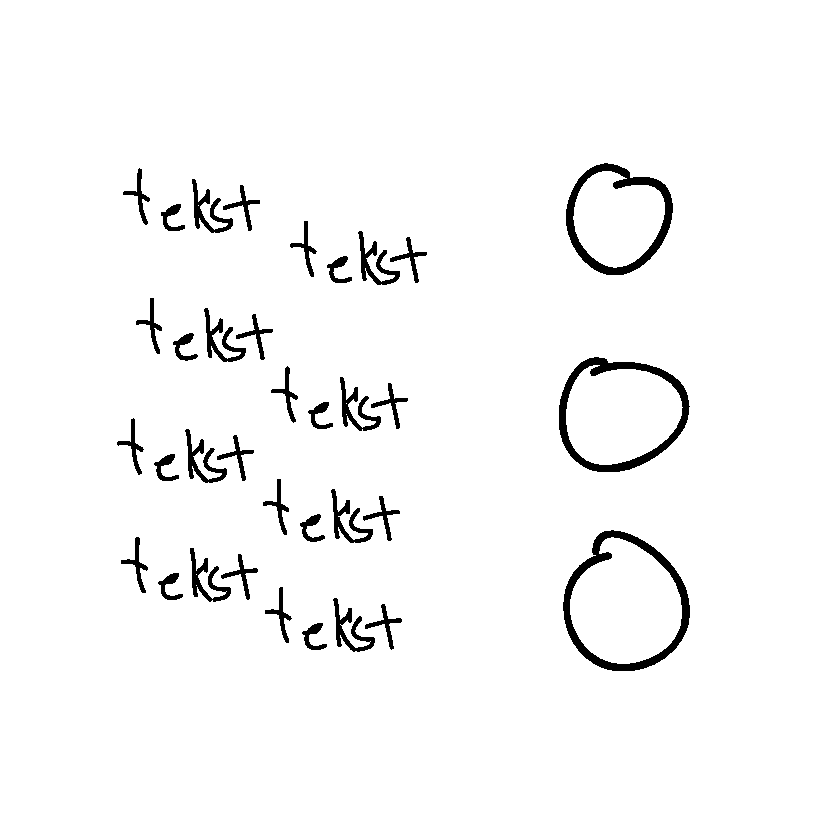
\includegraphics[scale=0.31]{img/boxinguden.pdf}\quad%
	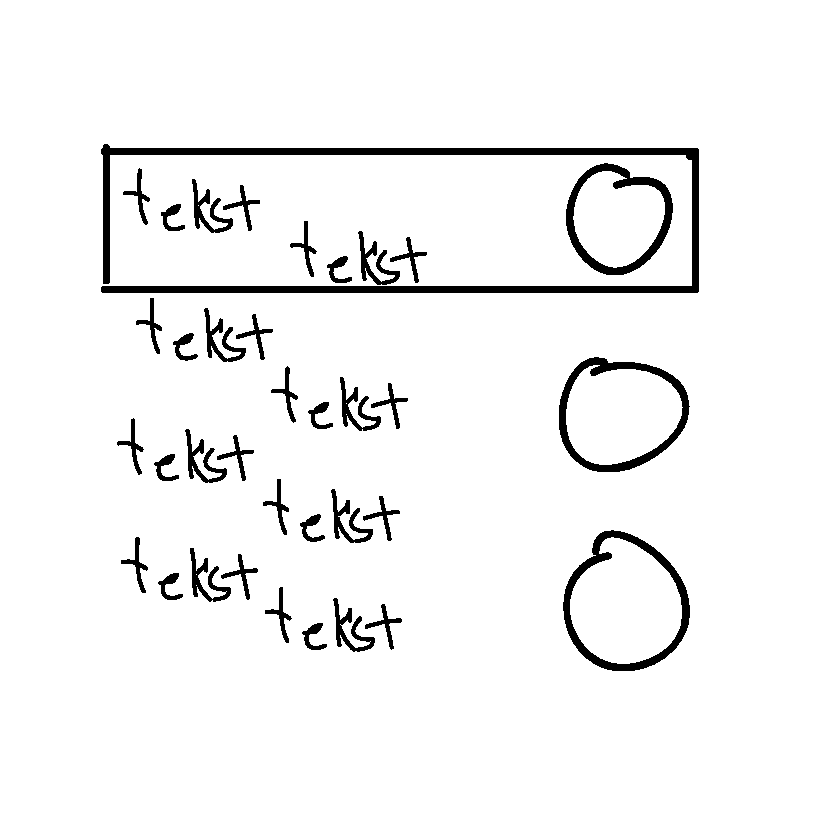
\includegraphics[scale=0.31]{img/boxingmed.pdf}
\end{frame}

\section{Sketching \& Prototyping}

\begin{frame}{Ideation}
		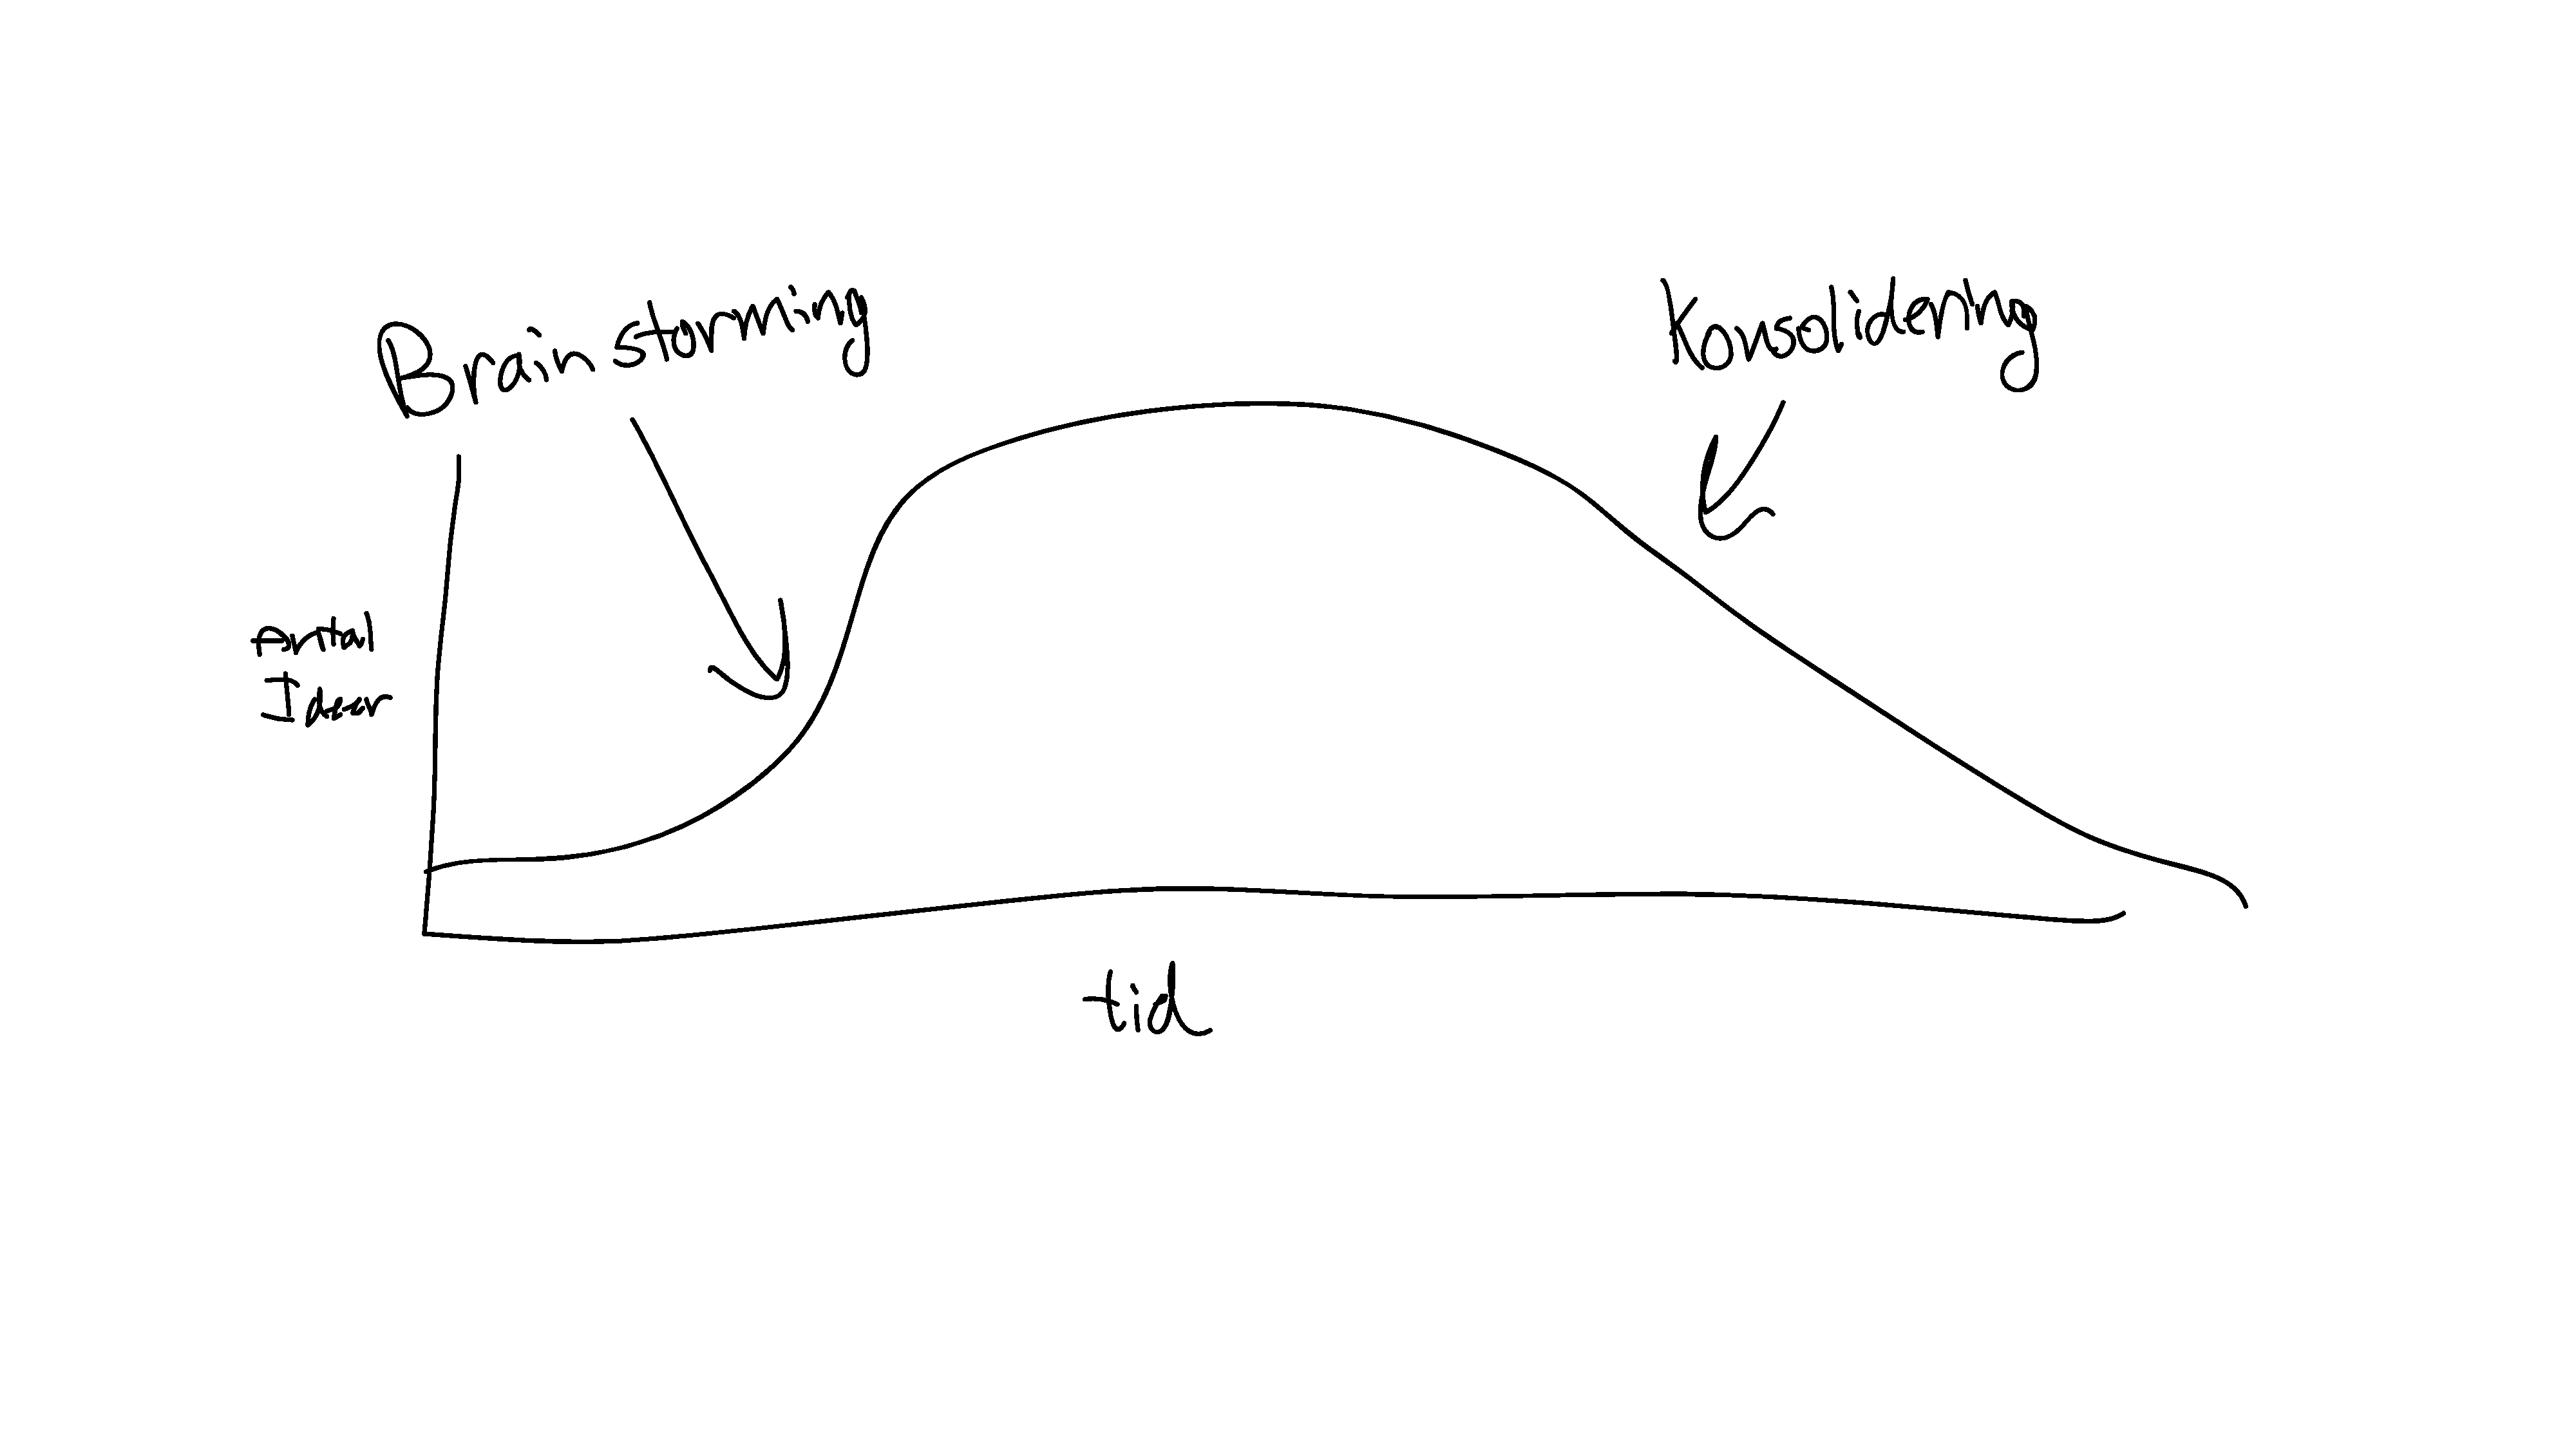
\includegraphics[scale=0.18]{img/ideation.pdf}
\end{frame}

\begin{frame}{Hvad er en sketch I}
	\centering
	\includegraphics[width=\linewidth]{img/operasketch.jpg}
\end{frame}

\begin{frame}{Hvad er en sketch II}
	\centering
	\includegraphics[width=\linewidth]{img/Sydney_opera_house.jpg}
\end{frame}

\begin{frame}{Hvad er prototyper I}
	\centering
	\includegraphics[width=\linewidth]{img/paperprotoyping.jpg}
\end{frame}

\begin{frame}{Hvad er prototyper II}
	\centering
	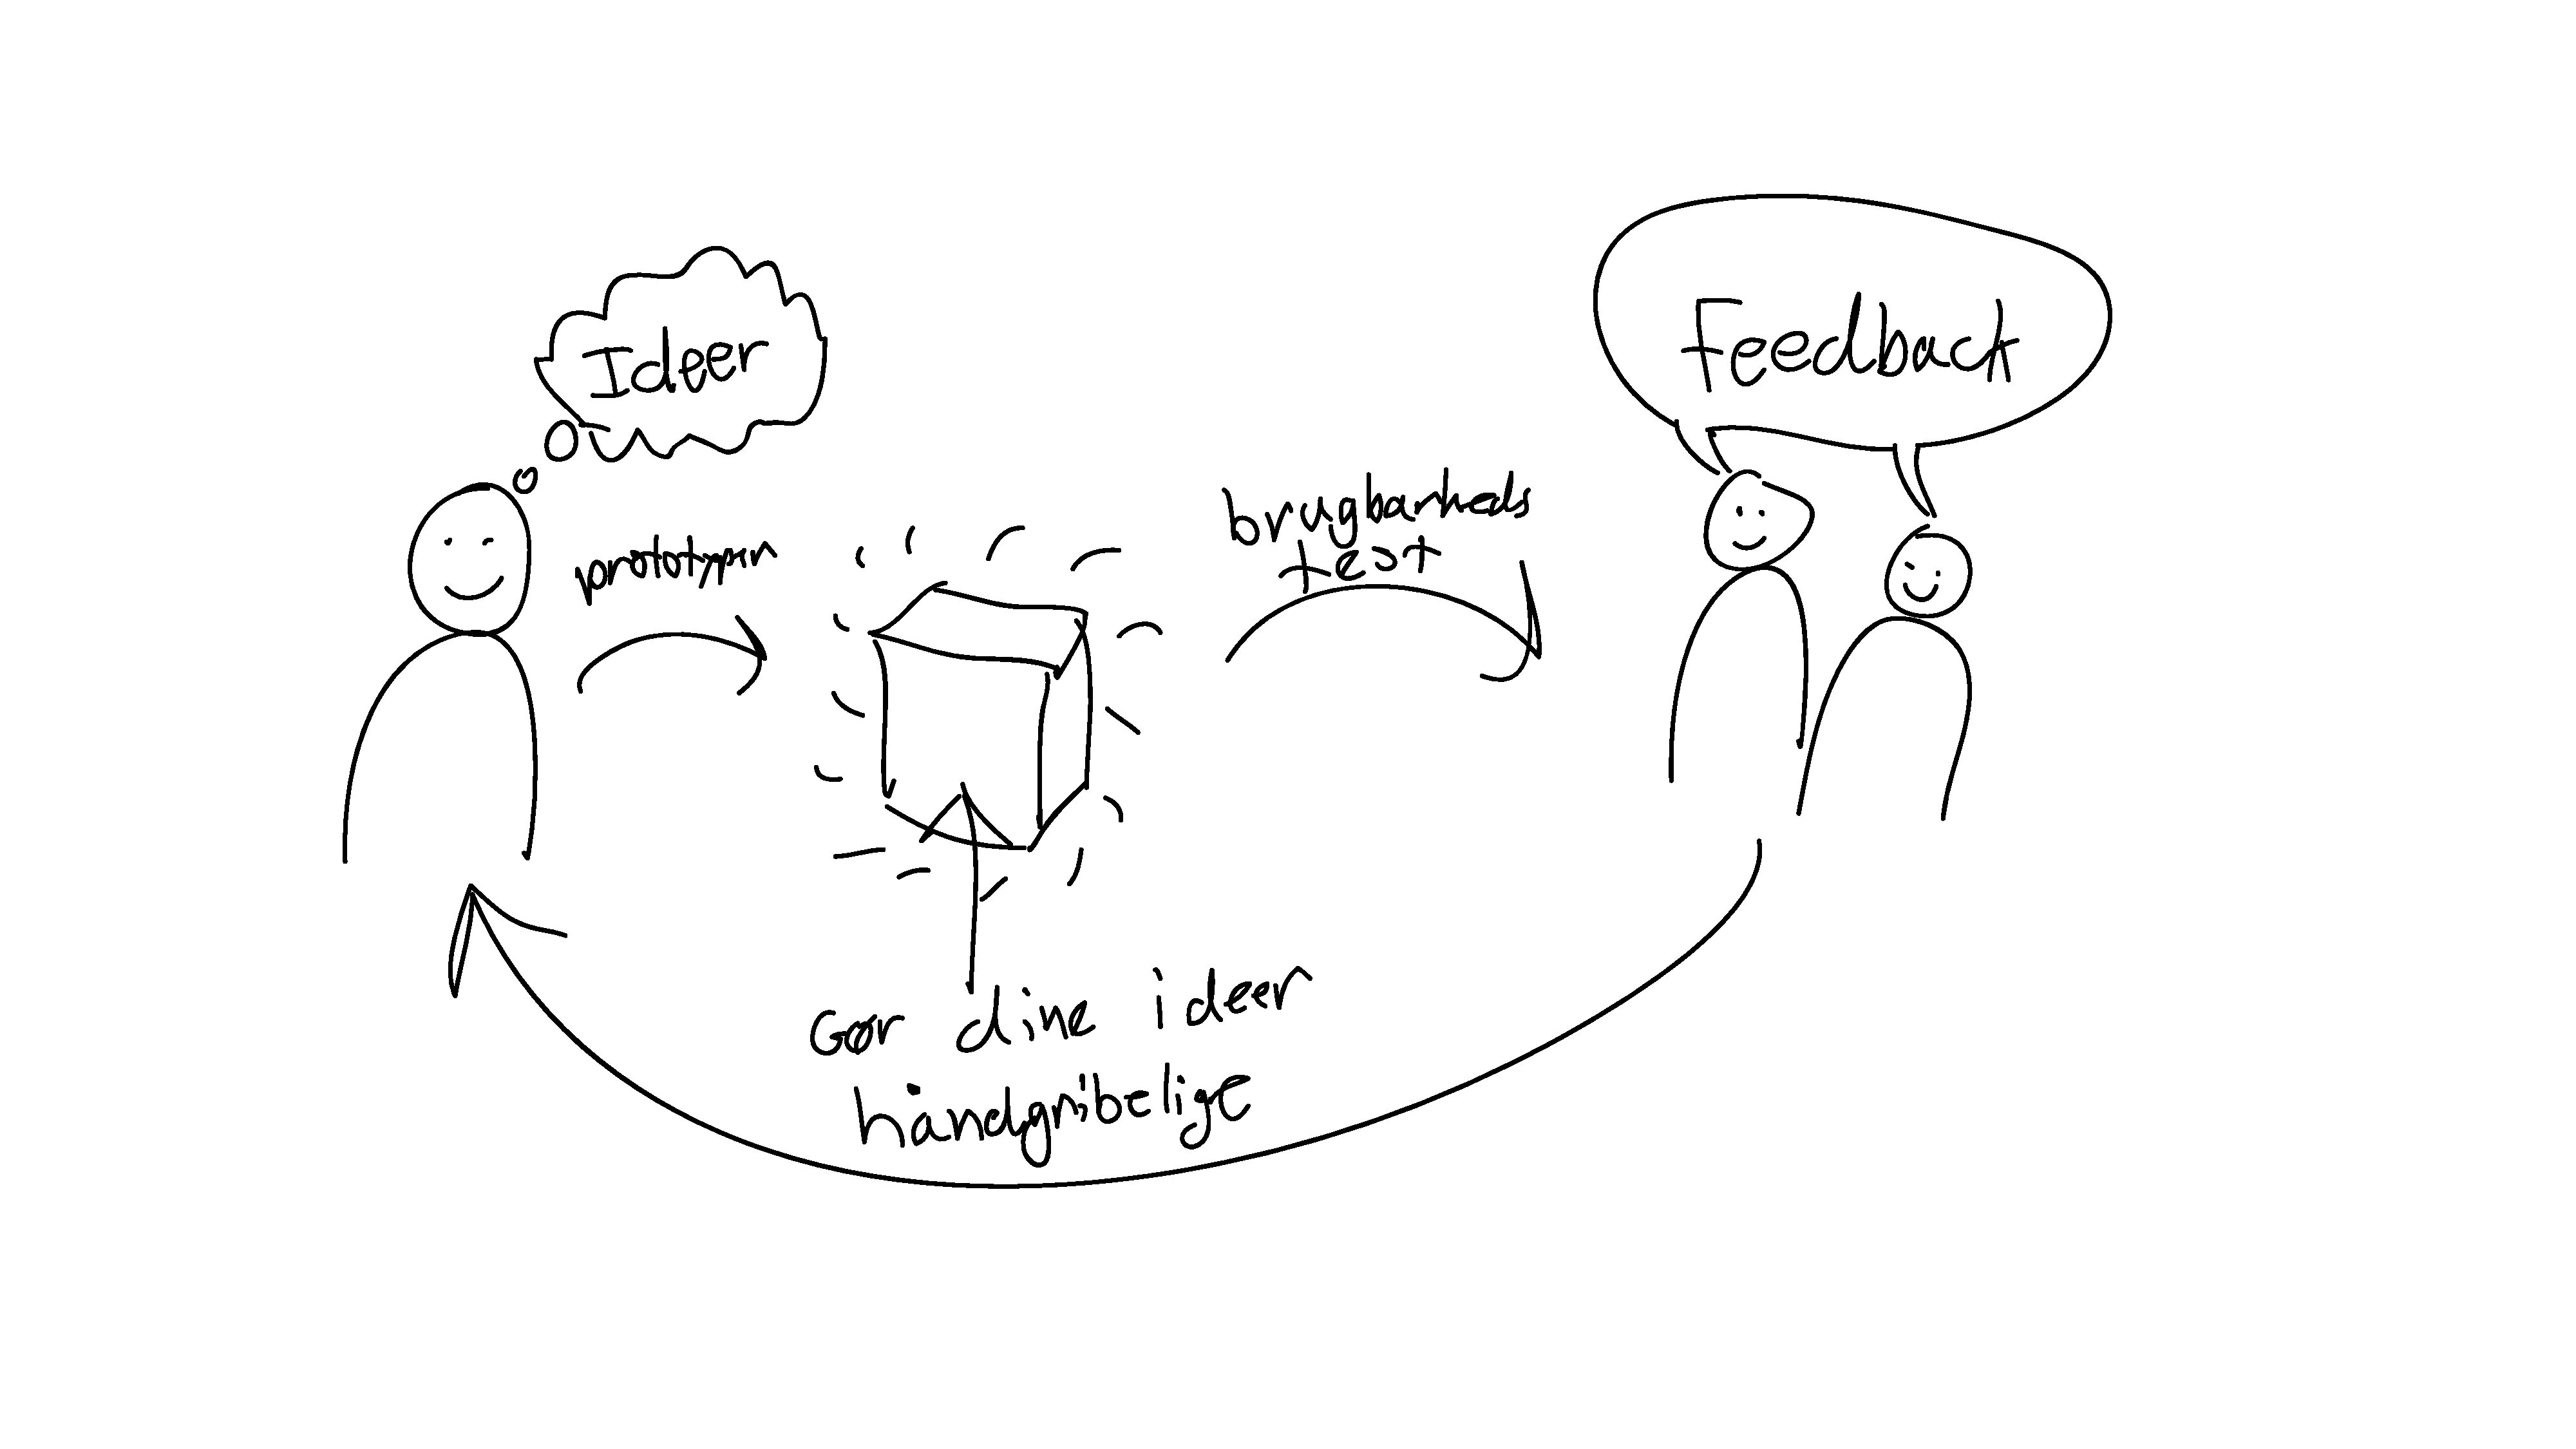
\includegraphics[scale=0.18]{img/prototypingloop.pdf}
\end{frame}

\begin{frame}{Sketch \& Prototype egenskaber}
\begin{center}
  \begin{tabular}{| l | l |}
    \hline
	\textbf{Sketch} & \textbf{Prototype} \\ \hline
    Hurtig & Knap så Hurtig\\ \hline
    Billig & Knap så Billig\\ \hline
    Talrige & Få \\ \hline
    Flertydige & Præcise \\ \hline
    Foreslår og udforsker & Uddyber \\ \hline
    Provokerer & Løser \\ \hline
    Giver spørgsmål & Giver svar \\ \hline
  \end{tabular}
\end{center}
\end{frame}

\plain{
Øvelse: 
Ide generation, Brainstorming.

Lav en masse sketches

f.eks. vejr app, trænings app, fifa kortsamler
 }

\begin{frame}{Prototyping Redskaber}
\centering
	\includegraphics[width=\linewidth]{img/tapeandtools.png}
\end{frame}

\begin{frame}{Prototyping Tricks}
\centering
	\includegraphics[width=\linewidth]{img/desktopsketch.png}
\end{frame}

\begin{frame}{Prototyping Tricks}
\centering
	\includegraphics[width=\linewidth]{img/pagessketch.png}
\end{frame}

\begin{frame}{Prototyping Tricks}
\centering
	\includegraphics[width=\linewidth]{img/sketchtricks.png}
\end{frame}

\begin{frame}{Prototyping Tricks}
\centering
	\includegraphics[width=\linewidth]{img/dropdown.png}
\end{frame}

\begin{frame}{Prototyping Tricks}
\centering
	\includegraphics[width=\linewidth]{img/expandablelists.png}
\end{frame}

\begin{frame}{Prototyping Tricks}
\centering
	\includegraphics[width=\linewidth]{img/prototypingswipe.jpg}
\end{frame}

\begin{frame}{Prototyping Tricks}
\centering
	\includegraphics[width=\linewidth]{img/prototypingflow.jpg}
\end{frame}

\begin{frame}{Prototyping Tricks}
\centering
	\includegraphics[width=\linewidth]{img/prototypingorganized.png}
\end{frame}

\begin{frame}{Prototyping Tricks}
\centering
	\includegraphics[width=\linewidth]{img/prototypingflip.jpg}
\end{frame}

\plain{
Øvelse:

Lav en prototype, hver, af jeres app ide
 
 }
 
\section{Brugbarhedstest}

\begin{frame}{Brugbarhed / Usability}
		\includegraphics[width=\linewidth]{img/carusability.jpg}
\end{frame}

\begin{frame}{Brugbarhed / Usability}
		\includegraphics[width=\linewidth]{img/observerusermoderator.png}
\end{frame}

\begin{frame}{Brugbarhed / Usability}
		\includegraphics[width=\linewidth]{img/tabletusability.jpg}
\end{frame}

\begin{frame}{Brugbarhedstest Aktiviteter}
	\begin{itemize}
		\item \textbf{Lav en testplan}
		\begin{itemize}
			\item Formålet med testen
			\item Hvem er vores brugere?
			\item Hvilke redskaber har vi?
			\item Hvordan skal vi teste?
			\item Fremstil opgaver der tester funktionaliteten
		\end{itemize}
		\item \textbf{Udfør testen}
			\begin{itemize}
				\item Præsenter din app
				\item Sæt testpersonen i gang med opgaver
				\item Noter problemer imens testpersonen løser opgaverne
			\end{itemize}
		\item \textbf{Gennemgå dit data, forbedrer din prototype og gentag}
	\end{itemize}

\end{frame}

\section{Appinventor}

\plain{
\url{http://appinventor.mit.edu/}
 }
 

\end{document}
